\begin{frame}
    \frametitle{Least Squares in General}
    \note{Excerpt from Cyrill Stachniss's course: https://youtu.be/r2cyMQ5NB1o?si=WYODHSkWun3FL7jR}
    
    Approach to compute a solution for an overdetermined system

    \begin{itemize}
        \item More equations than unknowns
        \item Minimizes the sum of squared errors in the equations
        \item Standard approach for a wide range of problems
        \item Used to estimate the parameter model given a set of observations
    \end{itemize}
\end{frame}

\begin{frame}
    \frametitle{Our Problem}
    \note{Excerpt from Cyrill Stachniss's course: https://youtu.be/r2cyMQ5NB1o?si=WYODHSkWun3FL7jR}
    
    Given a system described by a set of $n$ observation functions $\left\{f_{i}\left(\state\right)\right\}_{i=1:n}$

    \begin{itemize}
        \item $\stateBold$ is the state vector
        \item $\observationBold$ is a measurement of the state $\stateBold$
        \item $\prediction_{i} = f_{i}\left(\stateBold\right)$ is a function that maps the state $\stateBold$ to a predicted measurement $\prediction_{i}$
        \item Given $n$ noisy measurements $\observationBold_{1:n}$ about the state $\stateBold$
        \item Objective: Estimate the state $\stateBold$ that best explains the measurements $\observationBold_{1:n}$
    \end{itemize}

    \begin{center}
        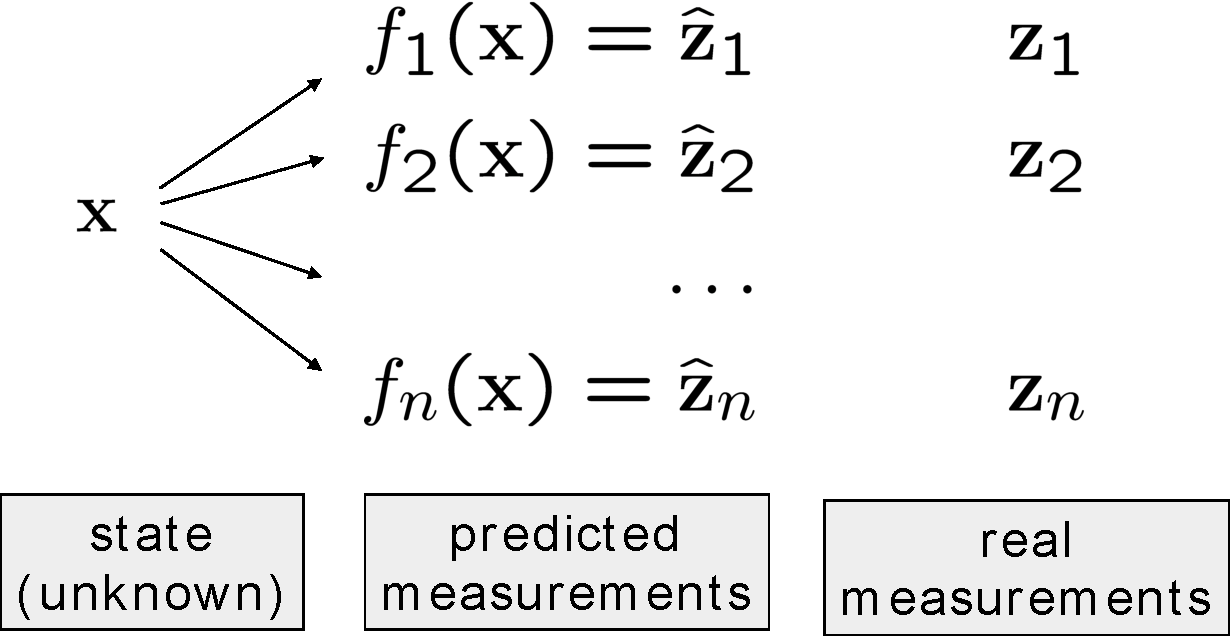
\includegraphics[width=0.5\textwidth]{images/least_squares.pdf}
    \end{center}

\end{frame}

\begin{frame}
    \frametitle{Example}
    \note{Excerpt from Cyrill Stachniss's course: https://youtu.be/r2cyMQ5NB1o?si=WYODHSkWun3FL7jR}
    
    \begin{center}
        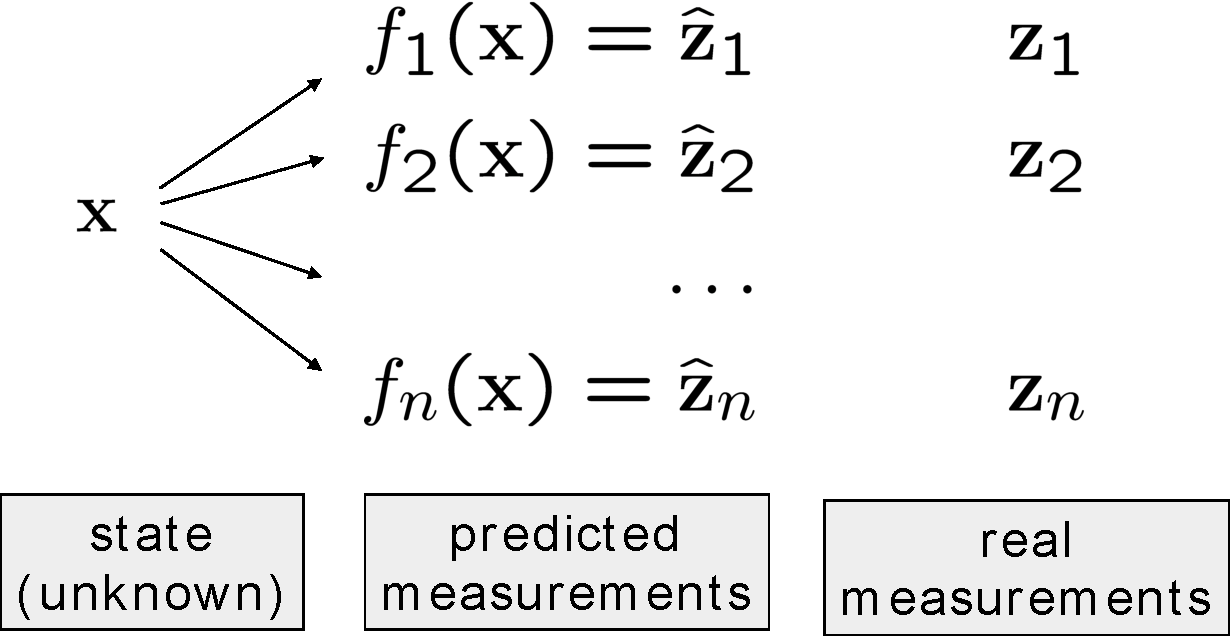
\includegraphics[width=0.7\textwidth]{images/least_squares.pdf}
    \end{center}
    
    \begin{itemize}
        \item $\stateBold$: 3D position of the points
        \item $\observationBold_{i}$: Coordinates of the 3D points projected onto the images
        \item Estimate the most likely 3D position of the points based on their projections in the images (given the camera poses)
    \end{itemize}
\end{frame}

\begin{frame}
    \frametitle{Error Function}
    \note{Excerpt from Cyrill Stachniss's course: https://youtu.be/r2cyMQ5NB1o?si=WYODHSkWun3FL7jR}
    
    \begin{itemize}
        \item The error $\error_{i}$ is typically the difference between the actual measurement and the prediction:
            \begin{equation*}
                \error_{i}\left( \stateBold \right) = \observationBold_{i} - f_{i}\left( \stateBold \right)
            \end{equation*}
        \item Assume the error follows a normal distribution with zero mean and covariance matrix $\covarianceBold_{i}$
        \item The Gaussian error information matrix is $\informationMatrix_{i} = \inverse{\covarianceBold_{i}}$
        \item The squared error of a measurement depends only on the state and is a scalar:
            \begin{equation*}
                \error_{i}\left( \stateBold \right) = \error_{i}\left( \stateBold \right)^{\top} \informationMatrix_{i} \error_{i}\left( \stateBold \right)
            \end{equation*}
    \end{itemize}
\end{frame}

\begin{frame}
    \frametitle{Objective: Find the Minimum}
    \note{Excerpt from Cyrill Stachniss's course: https://youtu.be/r2cyMQ5NB1o?si=WYODHSkWun3FL7jR}
    
    \begin{itemize}
        \item Find the state $\stateBold^{*}$ that minimizes the error given all measurements
        
        \begin{center}
            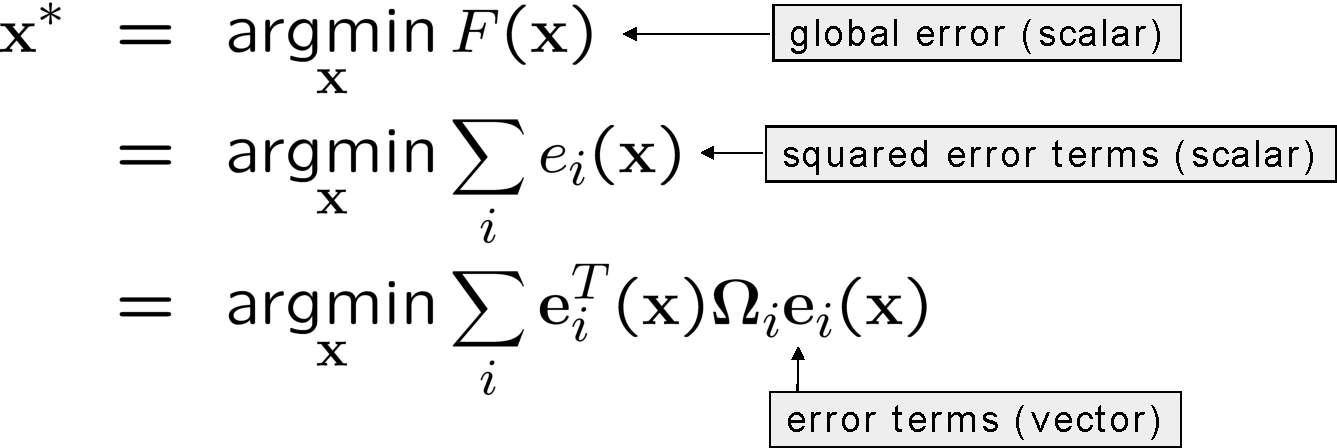
\includegraphics[width=0.7\textwidth]{images/find_minimum.pdf}
        \end{center}
    \end{itemize}

\end{frame}

\begin{frame}
    \frametitle{Objective: Find the Minimum}
    \note{Excerpt from Cyrill Stachniss's course: https://youtu.be/r2cyMQ5NB1o?si=WYODHSkWun3FL7jR}
    
    \begin{itemize}
        \item Find the state $\stateBold^{*}$ that minimizes the error given all measurements
        
        \begin{equation*}
            \stateBold^{*} = \argmin_{\stateBold} \sum_{i} \error_{i}\left( \stateBold \right)^{\top} \informationMatrix_{i} \error_{i}\left( \stateBold \right)
        \end{equation*}
        
        
        \item A general solution is to derive the global error function and find its zeros
        \item Often complex with no closed-form solution $\rightarrow$ Numerical methods
    \end{itemize}
    
\end{frame}


\begin{frame}
    \frametitle{Assumptions}
    \note{Excerpt from Cyrill Stachniss's course: https://youtu.be/r2cyMQ5NB1o?si=WYODHSkWun3FL7jR}
    \begin{itemize}
        \item A "good" initial solution is available
        \item The error functions are "smooth" near the minimum (ideally global)
        \item Thus, we can solve the problem using iterative local linearizations
    \end{itemize}

\end{frame}

\begin{frame}
    \frametitle{Solve Using Iterative Local Linearizations}
    \note{Excerpt from Cyrill Stachniss's course: https://youtu.be/r2cyMQ5NB1o?si=WYODHSkWun3FL7jR}
    \begin{itemize}
        \item Linearize the error terms around the current/initial solution
        \item Compute the first derivative of the squared error function
        \item Set to zero and solve the linear system
        \item Obtain the new state (hopefully closer to the minimum)
        \item Iterate
    \end{itemize}
\end{frame}

\begin{frame}
    \frametitle{Linearize the Error Function}
    \note{Excerpt from Cyrill Stachniss's course: https://youtu.be/r2cyMQ5NB1o?si=WYODHSkWun3FL7jR}
    
    \begin{itemize}
        \item We can approximate the error around an initial estimate $\stateBold$ using a Taylor expansion
    \end{itemize}
    
    \begin{equation*}
        \error_{i}(\stateBold + \vec{\Delta}\stateBold) \simeq  \underbrace{\error_{i}(\stateBold)}_{\error_{i}} + \jacobian_{i}\vec{\Delta}\stateBold \quad \text{with} \quad \jacobian_{i} = \dfrac{\partial\error_{i}(\stateBold)}{\partial\stateBold}
    \end{equation*}
    
\end{frame}

\begin{frame}
    \frametitle{Squared Error}
    \note{Excerpt from Cyrill Stachniss's course: https://youtu.be/r2cyMQ5NB1o?si=WYODHSkWun3FL7jR}
    
    \begin{itemize}
        \item With the above linearization, we can fix $\stateBold$ and perform minimization on the increments $\Delta\stateBold$
        \item Substitute the Taylor expansion into the squared error terms:
        \only<1>{
            \begin{align*}
                e_{i}(\stateBold + \vec{\Delta}\stateBold) &= \dots
            \end{align*}
        }
        \only<2>{
            \begin{align*}
                e_{i}(\stateBold + \vec{\Delta}\stateBold) &= \error_{i}\left( \stateBold + \Delta \stateBold \right)^{\top} \informationMatrix_{i} \error_{i}\left( \stateBold  + \Delta \stateBold \right)
            \end{align*}
        }
        \only<3>{
            \begin{align*}
                e_{i}(\stateBold + \vec{\Delta}\stateBold) &= \error_{i}\left( \stateBold + \Delta \stateBold \right)^{\top} \informationMatrix_{i} \error_{i}\left( \stateBold  + \Delta \stateBold \right)\\
                &\simeq \left( \error_{i} + \jacobian_{i} \Delta \stateBold \right)^{\top} \informationMatrix_{i} \left( \error_{i} + \jacobian_{i} \Delta \stateBold \right)
            \end{align*}
        }
        \only<4>{
            \begin{align*}
                e_{i}(\stateBold + \vec{\Delta}\stateBold) &= \error_{i}\left( \stateBold + \Delta \stateBold \right)^{\top} \informationMatrix_{i} \error_{i}\left( \stateBold  + \Delta \stateBold \right)\\
                &\simeq \left( \error_{i} + \jacobian_{i} \Delta \stateBold \right)^{\top} \informationMatrix_{i} \left( \error_{i} + \jacobian_{i} \Delta \stateBold \right)\\
                &= \error_{i}^{\top} \informationMatrix_{i} \error_{i} + \error_{i}^{\top} \informationMatrix_{i} \jacobian_{i} \Delta \stateBold + \Delta \stateBold^{\top} \jacobian_{i}^{\top} \informationMatrix_{i} \error_{i} +  \Delta \stateBold^{\top} \jacobian_{i}^{\top} \informationMatrix_{i} \jacobian_{i} \Delta \stateBold
            \end{align*}
        }
    \end{itemize}
\end{frame}

\begin{frame}
    \frametitle{Squared Error (cont.)}
    \note{Excerpt from Cyrill Stachniss's course: https://youtu.be/r2cyMQ5NB1o?si=WYODHSkWun3FL7jR}
    
    \begin{itemize}
        \item All terms are scalars, so transposition has no effect
        \item Grouping similar terms, we obtain:
        \only<1>{
            \begin{align*}
                e_{i}(\stateBold + \vec{\Delta}\stateBold) &\simeq \error_{i}^{\top} \informationMatrix_{i} \error_{i} + \error_{i}^{\top} \informationMatrix_{i} \jacobian_{i} \Delta \stateBold + \Delta \stateBold^{\top} \jacobian_{i}^{\top} \informationMatrix_{i} \error_{i} +  \Delta \stateBold^{\top} \jacobian_{i}^{\top} \informationMatrix_{i} \jacobian_{i} \Delta \stateBold
            \end{align*}
        }
        \only<2>{
            \begin{align*}
                e_{i}(\stateBold + \vec{\Delta}\stateBold) &\simeq \error_{i}^{\top} \informationMatrix_{i} \error_{i} + \error_{i}^{\top} \informationMatrix_{i} \jacobian_{i} \Delta \stateBold + \Delta \stateBold^{\top} \jacobian_{i}^{\top} \informationMatrix_{i} \error_{i} +  \Delta \stateBold^{\top} \jacobian_{i}^{\top} \informationMatrix_{i} \jacobian_{i} \Delta \stateBold \\
                &= \underbrace{\error_{i}^{\top} \informationMatrix_{i} \error_{i}}_{c_{i}} + 2 \underbrace{\error_{i}^{\top} \informationMatrix_{i} \jacobian_{i}}_{\linearSystemb^{\top}_{i}} \Delta \stateBold + \Delta \stateBold^{\top} \underbrace{\jacobian_{i}^{\top} \informationMatrix_{i} \jacobian_{i}}_{\linearSystemH_{i}} \Delta \stateBold
            \end{align*}
        }
        \only<3>{
            \begin{align*}
                e_{i}(\stateBold + \vec{\Delta}\stateBold) &\simeq \error_{i}^{\top} \informationMatrix_{i} \error_{i} + \error_{i}^{\top} \informationMatrix_{i} \jacobian_{i} \Delta \stateBold + \Delta \stateBold^{\top} \jacobian_{i}^{\top} \informationMatrix_{i} \error_{i} +  \Delta \stateBold^{\top} \jacobian_{i}^{\top} \informationMatrix_{i} \jacobian_{i} \Delta \stateBold \\
                &= \underbrace{\error_{i}^{\top} \informationMatrix_{i} \error_{i}}_{c_{i}} + 2 \underbrace{\error_{i}^{\top} \informationMatrix_{i} \jacobian_{i}}_{\linearSystemb^{\top}_{i}} \Delta \stateBold + \Delta \stateBold^{\top} \underbrace{\jacobian_{i}^{\top} \informationMatrix_{i} \jacobian_{i}}_{\linearSystemH_{i}} \Delta \stateBold \\
                &= c_{i} + 2 \linearSystemb^{\top}_{i} \Delta \stateBold + \Delta \stateBold^{\top} \linearSystemH_{i} \Delta \stateBold
            \end{align*}
        }
    \end{itemize}
    
    
\end{frame}

\begin{frame}
    \frametitle{Global Error}
    \note{Excerpt from Cyrill Stachniss's course: https://youtu.be/r2cyMQ5NB1o?si=WYODHSkWun3FL7jR}
    
    \begin{itemize}
        \item The global error is the sum of squared error terms corresponding to individual measurements
        \item Forms a new expression approximating the global error near the current solution $\stateBold$
    \end{itemize}
    
    \begin{align*}
        F\left(\stateBold + \Delta \stateBold \right) &= \sum_{i} e_{i}(\stateBold + \vec{\Delta}\stateBold)\\
        F\left(\stateBold + \Delta \stateBold \right) &\simeq \sum_{i} \left( c_{i} + 2 \linearSystemb^{\top}_{i} \Delta \stateBold + \Delta \stateBold^{\top} \linearSystemH_{i} \Delta \stateBold \right) \\
        &= \sum_{i} c_{i} + 2 \left( \sum_{i} \linearSystemb^{\top}_{i} \right) \Delta \stateBold + \Delta \stateBold^{\top} \left( \sum_{i} \linearSystemH_{i} \right) \Delta \stateBold
    \end{align*}
    
    
\end{frame}

\begin{frame}
    \frametitle{Global Error (cont.)}
    \note{Excerpt from Cyrill Stachniss's course: https://youtu.be/r2cyMQ5NB1o?si=WYODHSkWun3FL7jR}
    
    \begin{align*}
        F\left(\stateBold + \Delta \stateBold \right) &\simeq \sum_{i} \left( c_{i} + 2 \linearSystemb^{\top}_{i} \Delta \stateBold + \Delta \stateBold^{\top} \linearSystemH_{i} \Delta \stateBold \right) \\
        &= \underbrace{\sum_{i} c_{i}}_{c} + 2 \underbrace{\left( \sum_{i} \linearSystemb^{\top}_{i} \right)}_{\linearSystemb^{\top}} \Delta \stateBold + \Delta \stateBold^{\top} \underbrace{\left( \sum_{i} \linearSystemH_{i} \right)}_{\linearSystemH} \Delta \stateBold \\
        &= c + 2 \linearSystemb^{\top} \Delta \stateBold + \Delta \stateBold^{\top} \linearSystemH \Delta \stateBold
    \end{align*}
    
    with
    
    \begin{align*}
        \linearSystemb^{\top} &= \sum_{i} \error_{i}^{\top} \informationMatrix_{i} \jacobian_{i} \\ 
        \linearSystemH &= \sum_{i}  \jacobian_{i}^{\top} \informationMatrix_{i} \jacobian_{i}
    \end{align*}
    
    
\end{frame}

\begin{frame}
    \frametitle{Quadratic Form}
    \note{Excerpt from Cyrill Stachniss's course: https://youtu.be/r2cyMQ5NB1o?si=WYODHSkWun3FL7jR}
    
    \begin{itemize}
        \item<1-> We can write the global error terms as a quadratic form in $\Delta \stateBold$
        
        \begin{equation*}
            F\left(\stateBold + \Delta \stateBold \right) = c + 2 \linearSystemb^{\top} \Delta \stateBold + \Delta \stateBold^{\top} \linearSystemH \Delta \stateBold
        \end{equation*}
        
        \item<1> \alert{How to compute the minimum of a quadratic form?}
        \item<2-> Compute the derivative of $F\left(\stateBold + \Delta \stateBold \right)$ with respect to $\Delta \stateBold$ (given $\stateBold$)
        \item<2-> Differentiate and set to 0
        \item<2-> Solve
    \end{itemize}

\end{frame}

\begin{frame}
    \frametitle{Differentiating the Quadratic Form}
    \note{Excerpt from Cyrill Stachniss's course: https://youtu.be/r2cyMQ5NB1o?si=WYODHSkWun3FL7jR}
    
    \begin{itemize}
        \item Given the quadratic form
        \begin{equation*}
            f(\stateBold) = \stateBold^{\top} \linearSystemH \stateBold + \linearSystemb^{\top} \stateBold
        \end{equation*}
        \item The first derivative is
        \begin{equation*}
            \dfrac{\partial f}{\partial \stateBold} = \left( \linearSystemH + \linearSystemH^{\top} \right) \stateBold + \linearSystemb
        \end{equation*}
    \end{itemize}
    
    See: The Matrix Cookbook, section 2.4.2
   
\end{frame}

\begin{frame}
    \frametitle{Quadratic Form}
    \note{Excerpt from Cyrill Stachniss's course: https://youtu.be/r2cyMQ5NB1o?si=WYODHSkWun3FL7jR}
    
    \begin{itemize}
        \item We can write the global error terms as a quadratic form in $\Delta \stateBold$
        \begin{equation*}
            F\left(\stateBold + \Delta \stateBold \right) = c + 2 \linearSystemb^{\top} \Delta \stateBold + \Delta \stateBold^{\top} \linearSystemH \Delta \stateBold
        \end{equation*}
        \item The derivative of $F\left(\stateBold + \Delta \stateBold \right)$
        \begin{equation*}
            \dfrac{\partial F\left(\stateBold + \Delta \stateBold \right)}{\partial \Delta \stateBold} \simeq 2 \linearSystemb + 2 \linearSystemH \Delta \stateBold
        \end{equation*}
    \end{itemize}
    
\end{frame}

\begin{frame}
    \frametitle{Minimizing the Quadratic Form}
    \note{Excerpt from Cyrill Stachniss's course: https://youtu.be/r2cyMQ5NB1o?si=WYODHSkWun3FL7jR}
    
    \begin{itemize}
        \item Derivative of $F\left(\stateBold + \Delta \stateBold \right)$
        \begin{equation*}
            \dfrac{\partial F\left(\stateBold + \Delta \stateBold \right)}{\partial \Delta \stateBold} \simeq 2 \linearSystemb + 2 \linearSystemH \Delta \stateBold
        \end{equation*}
        \item Setting to 0
        \begin{equation*}
            0 = 2 \linearSystemb + 2 \linearSystemH \Delta \stateBold
        \end{equation*}
        \item Leads to the linear system
        \begin{equation*}
            \linearSystemH \Delta \stateBold = -\linearSystemb 
        \end{equation*}
        \item The solution for the increment $\Delta \stateBold^{*}$ is
        \begin{equation*}
             \Delta \stateBold^{*} = - \inverse{\linearSystemH} \linearSystemb 
        \end{equation*}
    \end{itemize}
    
\end{frame}

\begin{frame}
    \frametitle{Solution with Gauss-Newton}
    \note{Excerpt from Cyrill Stachniss's course: https://youtu.be/r2cyMQ5NB1o?si=WYODHSkWun3FL7jR}
    
    Iterate the following steps:
    \begin{itemize}
        \item Linearize around $\stateBold$ and compute for each measurement
        \begin{equation*}
            \error_{i}(\stateBold + \vec{\Delta}\stateBold) \simeq  \error_{i}(\stateBold) + \jacobian_{i}\vec{\Delta}\stateBold
        \end{equation*}
        \item Compute the terms of the linear system
        \begin{equation*}
            \linearSystemb^{\top} = \sum_{i} \error_{i}^{\top} \informationMatrix_{i} \jacobian_{i} \quad \quad \linearSystemH = \sum_{i} \jacobian_{i}^{\top} \informationMatrix_{i} \jacobian_{i}
        \end{equation*}
    \item Solve the linear system
    \begin{equation*}
        \Delta \stateBold^{*} = - \inverse{\linearSystemH} \linearSystemb 
    \end{equation*}
    \item Update the state
    \begin{equation*}
        \stateBold \leftarrow \stateBold + \Delta \stateBold^{*}
    \end{equation*} 
    \end{itemize}
    
\end{frame}

\begin{frame}
    \frametitle{Example: Odometry Calibration}
    \note{Excerpt from Cyrill Stachniss's course: https://youtu.be/r2cyMQ5NB1o?si=WYODHSkWun3FL7jR}
    
    \begin{itemize}
        \item Odometry measurements $\controlCommand_{i}$
        \item Remove systematic error through calibration
        \item Assumption: We have ground-truth odometry $\controlCommand_{i}^{*}$
        \item Ground-truth provided by systems: Motion Capture (Vicon), Scan-Matching, or SLAM
    \end{itemize}
    
\end{frame}

\begin{frame}
    \frametitle{Example: Odometry Calibration}
    \note{Excerpt from Cyrill Stachniss's course: https://youtu.be/r2cyMQ5NB1o?si=WYODHSkWun3FL7jR}
    
    \begin{itemize}
        \item There is a function $f_{i}(\stateBold)$ that, given some bias parameters $\stateBold$, returns a corrected (unbiased) odometry for the noisy reading $\controlCommand_{i}^{\prime}$ 
        \begin{equation*}
            \controlCommand_{i}^{\prime} = f_{i}(\stateBold) =
            \begin{bmatrix}
                x_{11} & x_{12} & x_{13} \\
                x_{21} & x_{22} & x_{23} \\
                x_{31} & x_{32} & x_{33}
            \end{bmatrix}
            \controlCommand_{i}
        \end{equation*}
    \item To obtain the correction function $f(\stateBold)$, we need to find the parameters $\stateBold$
    \end{itemize}
    
\end{frame}

\begin{frame}
    \frametitle{Odometry Calibration (cont.)}
    \note{Excerpt from Cyrill Stachniss's course: https://youtu.be/r2cyMQ5NB1o?si=WYODHSkWun3FL7jR}
    \begin{itemize}

        \item The state vector is 
        \begin{equation*}
            \stateBold =
            \begin{bmatrix}
                x_{11} & x_{12} & x_{13} & x_{21} & x_{22} & x_{23} & x_{31} & x_{32} & x_{33}
            \end{bmatrix}
        \end{equation*}
        \item The error function is
        \begin{equation*}
            \error_{i}(\stateBold) = \controlCommand_{i}^{*} - 
            \begin{bmatrix}
                x_{11} & x_{12} & x_{13} \\
                x_{21} & x_{22} & x_{23} \\
                x_{31} & x_{32} & x_{33}
            \end{bmatrix}
            \controlCommand_{i}
        \end{equation*}
        \item Its derivative is
        
        \begin{center}
            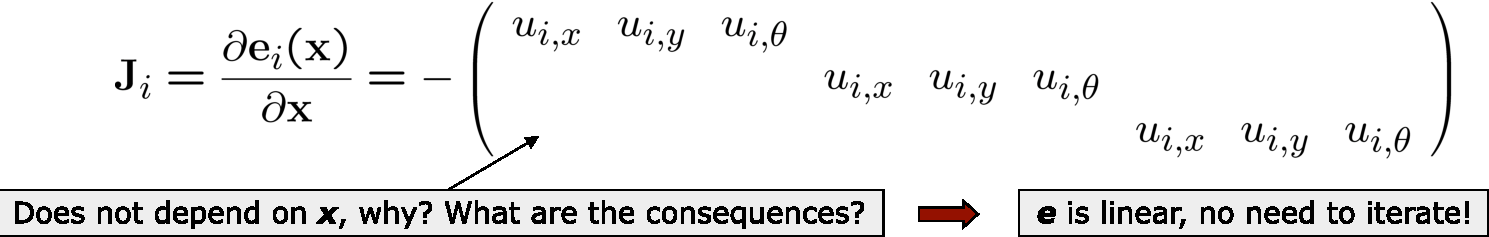
\includegraphics[width=0.8\columnwidth]{images/odometry_calibration_jacobian.pdf}
        \end{center}
        
        The fact that the first derivative (Jacobian) does not depend on $\stateBold$ is uncommon, as it means the error function $\error$ is linear!
        
        In this case, only one iteration is needed.

    \end{itemize}

    
\end{frame}

\begin{frame}
    \frametitle{Questions}
    \note{Excerpt from Cyrill Stachniss's course: https://youtu.be/r2cyMQ5NB1o?si=WYODHSkWun3FL7jR}
    
    \begin{itemize}
        \item<1-> What do the parameters look like if the odometry is perfect?
        \begin{itemize}
            \item<2-> The matrix should be the identity. Thus, the error is 0, and we have found the minimum.
        \end{itemize}
        \item<3-> How many measurements are needed to solve the calibration problem?
        \begin{itemize}
            \item<4-> We need to consider the number of unknown variables and the information provided by each observation. We have 9 unknowns. Each observation provides information about 3 variables (3 equations). Therefore, at least 3 observations are needed.
        \end{itemize}
        \item<5-> $\linearSystemH$ is symmetric. Why?
        \begin{itemize}
            \item<6-> $\linearSystemH$ is symmetric because $\linearSystemH = \jacobian^{\top}\Omega\jacobian$. $\Omega$ is symmetric positive definite, and $\jacobian$ is also symmetric, so the product is symmetric.
        \end{itemize}
        \item<7-> How does the structure of the measurement function affect the structure of $\linearSystemH$?
        \begin{itemize}
            \item<8-> $\linearSystemH$ is sparse because the Jacobians are sparse. The Jacobians are sparse because they encode how much information a measurement provides about all state variables. Thus, if our measurements only relate some variables (as in SLAM), $\linearSystemH$ will be sparse.
        \end{itemize}
    \end{itemize}

\end{frame}

\begin{frame}
    \frametitle{How to Efficiently Solve a Linear System?}
    \note{Excerpt from Cyrill Stachniss's course: https://youtu.be/r2cyMQ5NB1o?si=WYODHSkWun3FL7jR}
    \begin{itemize}
        \item Linear system $\linearSystemH \Delta \stateBold = -\linearSystemb$
        \item We can solve it using matrix inversion (in theory)
        \item In practice:
        \begin{itemize}
            \item Cholesky factorization
            \item QR decomposition
            \item Iterative methods like the Conjugate Gradient method (for large systems)
        \end{itemize}
        
    \end{itemize}
    
\end{frame}

\begin{frame}
    \frametitle{Cholesky Decomposition to Solve a Linear System}
    \note{Excerpt from Cyrill Stachniss's course: https://youtu.be/r2cyMQ5NB1o?si=WYODHSkWun3FL7jR}
    
    \begin{itemize}
        \item Let $\vec{A}$ be a symmetric positive definite matrix
        \item The system to solve is $\vec{A} \vec{x} = \vec{b}$
        \item Cholesky decomposition yields $\vec{A} = \vec{L} \vec{L}^{\top}$, where $\vec{L}$ is a lower triangular matrix
        \item<2> First solve
        \begin{equation*}
            \vec{L} \vec{y} = \vec{b}
        \end{equation*}
        \item<2> Then solve,
        \begin{equation*}
            \vec{L}^{\top} \vec{x} = \vec{y}
        \end{equation*}
    
    \end{itemize}
    
\end{frame}

\begin{frame}
    \frametitle{Gauss-Newton Summary}
    \note{Excerpt from Cyrill Stachniss's course: https://youtu.be/r2cyMQ5NB1o?si=WYODHSkWun3FL7jR}
    
    Method to minimize a squared error:
    \begin{itemize} 
        \item Start with an initial solution (initial guess)
        \item Linearize the individual error functions
        \item This leads to a quadratic form
        \item A linear system is obtained by differentiating and setting to 0
        \item Solving the linear system yields a state update
        \item Iterate
    \end{itemize}
    
\end{frame}

\begin{frame}
    \frametitle{Least Squares vs. Probabilistic State Estimation}
    \note{Excerpt from Cyrill Stachniss's course: https://youtu.be/r2cyMQ5NB1o?si=WYODHSkWun3FL7jR}
    
    \begin{itemize}
        \item So far, we minimized an error function
        \item How does this relate to state estimation in a probabilistic sense?
    \end{itemize}
    
\end{frame}

\begin{frame}
    \frametitle{Start with State Estimation}
    \note{Excerpt from Cyrill Stachniss's course: https://youtu.be/r2cyMQ5NB1o?si=WYODHSkWun3FL7jR}
    
    \begin{itemize}
        \item Bayes' rule, independence, and Markov assumptions allow us to rewrite
        \begin{equation*}
            p\left( \state_{0:t} | \observation_{1:t}, \controlCommand_{1:t} \right) = \eta p\left( \state_{0} \right) \prod_{t} \left[ p\left( \state_{t} | \state_{t-1}, \controlCommand_{t} \right) p\left( \observation_{t} | \state_{t} \right) \right]
        \end{equation*}
    \end{itemize}
    
    \note{p(x0) is a prior. Note that for x0, we have no observations or control commands.}
    
\end{frame}

\begin{frame}
    \frametitle{Log Likelihood}
    \note{Excerpt from Cyrill Stachniss's course: https://youtu.be/r2cyMQ5NB1o?si=WYODHSkWun3FL7jR}
    
    \begin{itemize}
        \item Rewriting as the log likelihood leads to
        \begin{equation*}
            \log p\left( \state_{0:t} | \observation_{1:t}, \controlCommand_{1:t} \right) = \text{const.}  \log p\left( \state_{0} \right) + \sum_{t} \left[ \log p\left( \state_{t} | \state_{t-1}, \controlCommand_{t} \right) + \log p\left( \observation_{t} | \state_{t} \right) \right]
        \end{equation*}
    \end{itemize}
    
\end{frame}

\begin{frame}
    \frametitle{Gaussian Assumption}
    \note{Excerpt from Cyrill Stachniss's course: https://youtu.be/r2cyMQ5NB1o?si=WYODHSkWun3FL7jR}
    
    \begin{itemize}
        \item Assuming Gaussian distribution
        \begin{equation*}
            \log p\left( \state_{0:t} | \observation_{1:t}, \controlCommand_{1:t} \right) = \text{const.}  \log \underbrace{p\left( \state_{0} \right)}_{\mathcal{N}} + \sum_{t} \left[ \log \underbrace{p\left( \state_{t} | \state_{t-1}, \controlCommand_{t} \right)}_{\mathcal{N}} + \log \underbrace{p\left( \observation_{t} | \state_{t} \right)}_{\mathcal{N}} \right]
        \end{equation*}
    \end{itemize}
    
\end{frame}

\begin{frame}
    \frametitle{Log of a Gaussian}
    \note{Excerpt from Cyrill Stachniss's course: https://youtu.be/r2cyMQ5NB1o?si=WYODHSkWun3FL7jR}

    
    \begin{itemize}
        \item The probability density function of the normal distribution is defined as
        \begin{equation*}
            p(x)=\det(2\pi\covariance)^{\frac{1}{2}} \exp\left(-\dfrac{1}{2} (x - \mu )^{\top} \inverse{\covariance} (x - \mu )  \right)
        \end{equation*}
        
        \item Log likelihood of a Gaussian
        \begin{equation*}
            \log \mathcal{N}(x; \mu, \Sigma) =  \text{const.} - \dfrac{1}{2} (x - \mu)^{\top} \inverse{\Sigma} (x - \mu)
        \end{equation*}
    \end{itemize}
    
\end{frame}

\begin{frame}
    \frametitle{Error Function as Exponent}
    \note{Excerpt from Cyrill Stachniss's course: https://youtu.be/r2cyMQ5NB1o?si=WYODHSkWun3FL7jR}
    
    \begin{itemize}
        \item Log likelihood of a Gaussian
        \begin{equation*}
            \log \mathcal{N}(x; \mu, \Sigma) =  \text{const.} - \dfrac{1}{2} \underbrace{\underbrace{(x - \mu)^{\top}}_{\error^{\top}(x)} \underbrace{\inverse{\Sigma}}_{\informationMatrix} \underbrace{(x - \mu)}_{\error(x)}}_{e(x)}
        \end{equation*}
        \item is equivalent, up to a constant, to the error functions used earlier
    \end{itemize}
    
\end{frame}

\begin{frame}
    \frametitle{Log Likelihood with Error Terms}
    \note{Excerpt from Cyrill Stachniss's course: https://youtu.be/r2cyMQ5NB1o?si=WYODHSkWun3FL7jR}
    
    \begin{itemize}
        \item Assuming Gaussian distribution
        \begin{equation*}
            \log p\left( \state_{0:t} | \observation_{1:t}, \controlCommand_{1:t} \right) = \text{const.} - \dfrac{1}{2} e_{p}(\state) -  \dfrac{1}{2} \sum_{t} \left[ e_{\controlCommand_{t}}(\state) + e_{\observation_{t}}(\state)\right]
        \end{equation*}
    \end{itemize}
    
\end{frame}

\begin{frame}
    \frametitle{Log Likelihood with Error Terms}
    \note{Excerpt from Cyrill Stachniss's course: https://youtu.be/r2cyMQ5NB1o?si=WYODHSkWun3FL7jR}
    
    \begin{itemize}
        \item Assuming Gaussian distribution
        \begin{equation*}
            \log p\left( \state_{0:t} | \observation_{1:t}, \controlCommand_{1:t} \right) = \text{const.} - \dfrac{1}{2} e_{p}(\state) -  \dfrac{1}{2} \sum_{t} \left[ e_{\controlCommand_{t}}(\state) + e_{\observation_{t}}(\state)\right]
        \end{equation*}
    \end{itemize}
    
\end{frame}

\begin{frame}
    \frametitle{Maximizing the Log Likelihood}
    \note{Excerpt from Cyrill Stachniss's course: https://youtu.be/r2cyMQ5NB1o?si=WYODHSkWun3FL7jR}
    
    \begin{itemize}
        \item Assuming Gaussian distribution
        \begin{equation*}
            \log p\left( \state_{0:t} | \observation_{1:t}, \controlCommand_{1:t} \right) = \text{const.} - \dfrac{1}{2} e_{p}(\state) -  \dfrac{1}{2} \sum_{t} \left[ e_{\controlCommand_{t}}(\state) + e_{\observation_{t}}(\state)\right]
        \end{equation*}
        \item Maximizing the log likelihood leads to 
        \begin{equation*}
            \argmax \log p\left( \state_{0:t} | \observation_{1:t}, \controlCommand_{1:t} \right) = \argmin e_{p}(\state) + \sum_{t} \left[ e_{\controlCommand_{t}}(\state) + e_{\observation_{t}}(\state)\right]
        \end{equation*}
    \end{itemize}
    
    
\end{frame}

\begin{frame}
    \frametitle{Minimizing the Squared Error is Equivalent to Maximizing the Log Likelihood of Independent Gaussian Distributions}
    \note{Excerpt from Cyrill Stachniss's course: https://youtu.be/r2cyMQ5NB1o?si=WYODHSkWun3FL7jR}
    \begin{itemize}
        \item With individual error terms for controls, measurements, and a prior:
        \begin{equation*}
            \argmax \log p\left( \state_{0:t} | \observation_{1:t}, \controlCommand_{1:t} \right) = \argmin e_{p}(\state) + \sum_{t} \left[ e_{\controlCommand_{t}}(\state) + e_{\observation_{t}}(\state)\right]
        \end{equation*}
    \end{itemize}
    
\end{frame}

\begin{frame}
    \frametitle{Summary}
    \note{Excerpt from Cyrill Stachniss's course: https://youtu.be/r2cyMQ5NB1o?si=WYODHSkWun3FL7jR}
    
    \begin{itemize}
        \item Technique for minimizing quadratic error functions
        \item Gauss-Newton is an iterative approach for nonlinear problems
        \item Uses linearization (approximation!)
        \item Equivalent to maximizing the log likelihood of independent Gaussians
        \item Popular method in many disciplines.
    \end{itemize}

    
\end{frame}

\begin{frame}
    \frametitle{Gauss-Newton Bibliography}
    \note{Excerpt from Cyrill Stachniss's course: https://youtu.be/r2cyMQ5NB1o?si=WYODHSkWun3FL7jR}
    \begin{itemize}
        \item Chapter 11.4 of \cite{thrun2005probabilistic}
    \end{itemize}
\end{frame}
